\documentclass[11pt,a4paper]{article}

\usepackage[margin=2.4cm]{geometry}
\usepackage{amsmath,amssymb,amsthm,mathtools}
\usepackage{enumitem}
\usepackage{booktabs}
\usepackage{array}
\usepackage{longtable}
\usepackage{tikz}
\usetikzlibrary{automata,positioning,arrows.meta,calc}
\usepackage{microtype}
\usepackage[hidelinks]{hyperref}
\usepackage{fancyhdr}
\usepackage{xcolor}

\usepackage{setspace}
\usepackage[breakable,skins]{tcolorbox}
\usepackage{titlesec}

\setstretch{1.2}
\setlength{\parskip}{0.75em}
\setlength{\parindent}{0pt}
\setlist{itemsep=0.35em,topsep=0.5em}
\setlength{\abovedisplayskip}{10pt}
\setlength{\belowdisplayskip}{10pt}
\renewcommand{\arraystretch}{1.3}
\titlespacing*{\paragraph}{0pt}{1.1em}{0.6em}
\titleformat{\section}{\Large\bfseries\color{blue!45!black}}{\thesection}{0.8em}{}[\vspace{0.2em}\titlerule]
\titlespacing*{\section}{0pt}{1.5em}{1.2em}

\tikzset{tm/.style={->,>=Stealth,shorten >=1pt,auto,semithick,
    every state/.style={draw,minimum size=9mm,inner sep=1pt,fill=blue!5},
    every node/.append style={font=\small},
    every loop/.style={looseness=6}},
  lab/.style={align=center,font=\footnotesize}}
\newcommand{\eps}{\varepsilon}
\newcommand{\blank}{\sqcup}
\newcommand{\enc}[1]{\langle #1\rangle}
\newcommand{\comp}[1]{\overline{#1}}
\newcommand{\Atm}{A_{\mathrm{TM}}}
\newcommand{\Etm}{E_{\mathrm{TM}}}
\newcommand{\HALTtm}{\mathit{HALT}_{\mathrm{TM}}}
\newcommand{\EQtm}{\mathit{EQ}_{\mathrm{TM}}}
\newcommand{\redm}{\le_{m}}
\newtcolorbox{questionbox}[1]{enhanced,breakable,colback=white,colframe=black!45,colbacktitle=black!8,coltitle=black,
  boxrule=0.6pt,arc=2pt,left=8pt,right=8pt,top=6pt,bottom=6pt,
  fonttitle=\bfseries,title={Question #1}}
\newenvironment{question}[1]{\par\bigskip\phantomsection
  \addcontentsline{toc}{section}{Q#1}\begin{questionbox}{#1}}{\end{questionbox}}
\newenvironment{soln}{\par\medskip{\large\bfseries Solution.}\par\smallskip}{\par\bigskip
  \noindent{\color{black!25}\rule{\linewidth}{0.4pt}}\par\medskip}

\pagestyle{fancy}
\fancyhf{}
\setlength{\headheight}{14pt}
\lhead{MTL783}
\rhead{Tutorial Sheet 3 -- Solutions}
\cfoot{\thepage}

\title{\textbf{MTL783: Tutorial Sheet 3}\\[0.3em]\large Complete solutions}
\date{}

\begin{document}
{\centering\Large\bfseries MTL783 -- Tutorial Sheet 3: Solutions\par}

\begin{question}{1}
Give the formal definition of a deterministic Turing machine. Explain the role of the transition function and describe how a transition changes the tape contents, head position, and current state.
\end{question}
\begin{soln}
A (deterministic) Turing machine is a 7-tuple
\[
M=(Q,\Sigma,\Gamma,\delta,q_0,q_{\mathrm{accept}},q_{\mathrm{reject}})
\]
where $Q,\Sigma,\Gamma$ are finite sets and
\begin{itemize}
\item $Q$ is the set of states, $q_0\in Q$ the start state, $q_{\mathrm{accept}}\neq q_{\mathrm{reject}}$ the accept and reject states;
\item $\Sigma$ is the input alphabet, with the blank $\blank\notin\Sigma$;
\item $\Gamma\supseteq\Sigma\cup\{\blank\}$ is the tape alphabet;
\item $\delta: Q\times\Gamma\to Q\times\Gamma\times\{L,R\}$ is the transition function.
\end{itemize}

\textbf{Role of $\delta$.} $\delta$ is the entire ``program''. In state $q$ reading symbol $a$, the rule $\delta(q,a)=(r,b,D)$ says:
\begin{enumerate}
\item \emph{tape:} overwrite the scanned $a$ with $b$ (only this cell changes);
\item \emph{head:} move one cell left ($D=L$) or right ($D=R$); a left move on the leftmost cell leaves the head where it is;
\item \emph{state:} go to state $r$.
\end{enumerate}
Since $\delta$ is a function, there is exactly one next move: the machine is deterministic.

\textbf{Configurations.} Write $u\,q\,av$ for ``tape $uav$, state $q$, head on $a$''. Then
\[
u\,q\,av \;\vdash\; u\,b\,r\,v \quad\text{if } D=R,
\qquad
uc\,q\,av \;\vdash\; u\,r\,cbv \quad\text{if } D=L .
\]
The machine starts in $q_0w$ (input $w$ on the leftmost cells, rest blank) and stops as soon as it enters $q_{\mathrm{accept}}$ or $q_{\mathrm{reject}}$. It accepts $w$ if it eventually reaches $q_{\mathrm{accept}}$; it may also run forever.
\end{soln}

\begin{question}{2}
Answer the following questions about Turing machines:
(1) Can the description of a Turing machine be written as a string?
(2) Is the number of Turing machines finite, countable, or uncountable?
(3) Can infinitely many strings represent the same TM?
\end{question}
\begin{soln}
\textbf{(1) Yes.} A TM is a finite object: finitely many states and symbols and a finite table $\delta$. Number the states $1,\dots,|Q|$ and the symbols $1,\dots,|\Gamma|$, and write each rule $\delta(q_i,a_j)=(q_k,a_l,D)$ as, e.g.,
\[
0^i\,1\,0^j\,1\,0^k\,1\,0^l\,1\,0^{D}
\qquad (D=1 \text{ for } L,\ D=2 \text{ for } R),
\]
separating rules by $11$. The result is a binary string $\enc{M}$.

\textbf{(2) Countably infinite.}
\emph{Infinite:} for every $n$ there is a machine with $n$ states.
\emph{Countable:} $M\mapsto\enc{M}$ is one-to-one into $\{0,1\}^*$, and $\{0,1\}^*$ is countable (list strings by length, then lexicographically). So there are not uncountably many.

\textbf{(3) Yes.} Renaming states, reordering the rules in the encoding, or adding extra states that are never entered all give different strings for a machine that behaves the same way. Adding $k$ such unused states for $k=1,2,3,\dots$ already gives infinitely many different encodings of machines that recognise the same language.
\end{soln}

\begin{question}{3}
Construct a Turing machine that decides the language $L=\{0^n1^n\mid n\ge 0\}$.
\end{question}
\begin{soln}
\textbf{Idea.} Match the 0s and 1s in pairs: cross off the leftmost $0$ (write $x$) and the leftmost $1$ (write $y$), return, repeat. When no $0$ is left, only $y$'s may remain.

\begin{center}
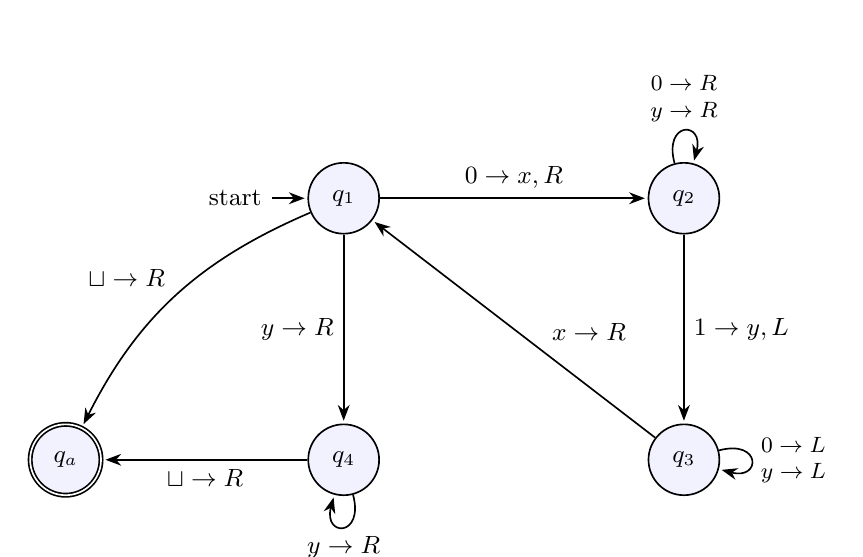
\begin{tikzpicture}[tm,node distance=3.4cm]
\node[state,initial] (q1) {$q_1$};
\node[state,right=of q1] (q2) {$q_2$};
\node[state,below=2.4cm of q2] (q3) {$q_3$};
\node[state,below=2.4cm of q1] (q4) {$q_4$};
\node[state,accepting,left=2.6cm of q4] (qa) {$q_{a}$};
\path
 (q1) edge node {$0\to x,R$} (q2)
 (q2) edge[loop above] node[lab] {$0\to R$\\ $y\to R$} ()
 (q2) edge node {$1\to y,L$} (q3)
 (q3) edge[loop right] node[lab] {$0\to L$\\ $y\to L$} ()
 (q3) edge node[swap,pos=0.4] {$x\to R$} (q1)
 (q1) edge node[swap] {$y\to R$} (q4)
 (q4) edge[loop below] node {$y\to R$} ()
 (q4) edge node {$\blank\to R$} (qa)
 (q1) edge[bend right=20] node[swap] {$\blank\to R$} (qa);
\end{tikzpicture}

{\footnotesize Missing transitions go to $q_{\mathrm{reject}}$. ``$a\to b,D$'' = read $a$, write $b$, move $D$; ``$a\to D$'' leaves $a$ unchanged.}
\end{center}

\begin{itemize}
\item $q_1$: at the leftmost unmatched symbol. A $0$ is crossed and we look for its $1$. A $y$ means all 0s are used: go to $q_4$ to check that only $y$'s remain. A blank means the input was empty: accept.
\item $q_2$: move right over $0$'s and $y$'s to the first $1$ and cross it. (Reaching $\blank$ or $x$ here = no matching 1: reject.)
\item $q_3$: move back left to the rightmost $x$, step right, repeat.
\item $q_4$: accept iff we see only $y$'s and then a blank. (A $0$ or $1$ here means unequal counts or wrong order: reject.)
\end{itemize}

\textbf{Why it decides $L$.} Each round crosses one $0$ and one $1$, and $q_2$ only skips $0$'s and $y$'s, so a $1$ can never appear before a $0$ without causing a rejection. Every round removes two unmarked symbols, so there are at most $n$ rounds, each of finite length: the machine always halts.

\textbf{Trace on $0011$:}
$q_1 0011\vdash x q_2 011\vdash x0q_2 11\vdash xq_3 0y1\vdash q_3x0y1\vdash xq_1 0y1\vdash\cdots\vdash xxyq_2 1\vdash\cdots\vdash xxq_1 yy\vdash xxyq_4y\vdash xxyyq_4\blank\vdash$ accept.
On $001$ the second round reaches $\blank$ in $q_2$ and rejects.
\end{soln}

\begin{question}{4}
Design a Turing machine that decides the language of palindromes over $\{0,1\}$:
$L=\{w\in\{0,1\}^*\mid w=w^R\}$.
\end{question}
\begin{soln}
\textbf{Idea.} Compare the outermost symbols. Erase the first symbol and \emph{remember it in the state}, run to the end, check the last symbol is the same and erase it, return, repeat. Accept when at most one symbol is left.

\begin{center}
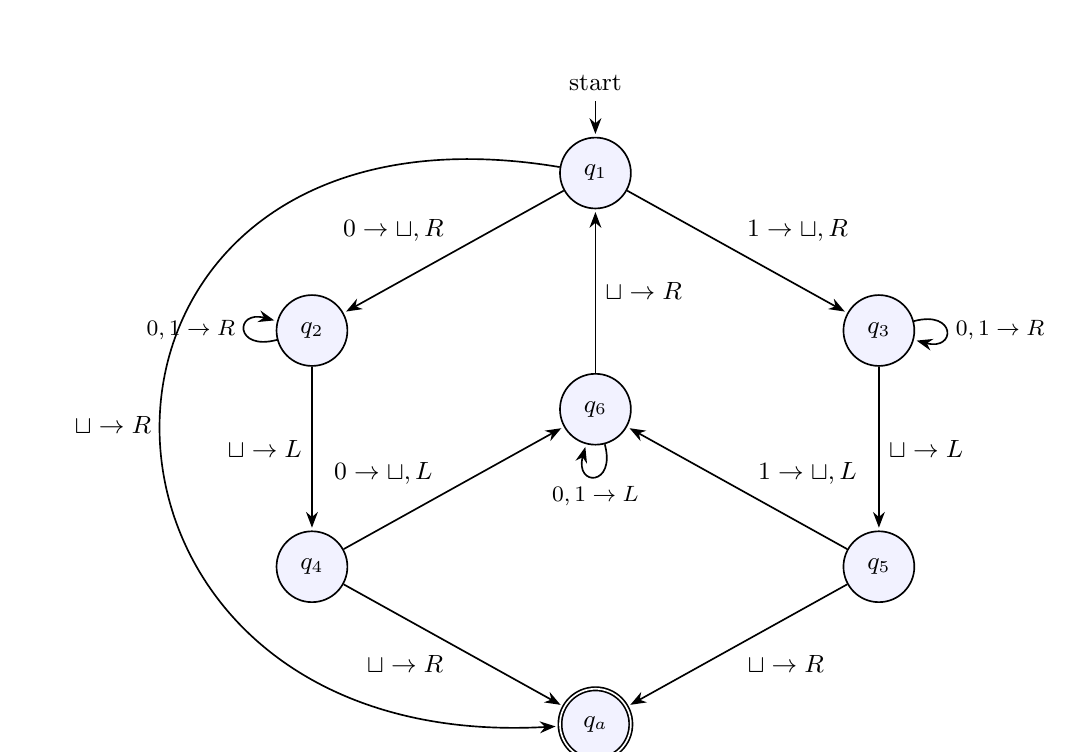
\begin{tikzpicture}[tm]
\node[state,initial above] (q1) at (0,0) {$q_1$};
\node[state] (q2) at (-3.6,-2) {$q_2$};
\node[state] (q3) at (3.6,-2) {$q_3$};
\node[state] (q4) at (-3.6,-5) {$q_4$};
\node[state] (q5) at (3.6,-5) {$q_5$};
\node[state] (q6) at (0,-3) {$q_6$};
\node[state,accepting] (qa) at (0,-7) {$q_a$};
\path
 (q1) edge[swap] node {$0\to\blank,R$} (q2)
 (q1) edge node {$1\to\blank,R$} (q3)
 (q2) edge[loop left] node[lab] {$0,1\to R$} ()
 (q3) edge[loop right] node[lab] {$0,1\to R$} ()
 (q2) edge[swap] node {$\blank\to L$} (q4)
 (q3) edge node {$\blank\to L$} (q5)
 (q4) edge node[pos=0.45] {$0\to\blank,L$} (q6)
 (q5) edge[swap] node[pos=0.45] {$1\to\blank,L$} (q6)
 (q6) edge[loop below] node[lab] {$0,1\to L$} ()
 (q6) edge[swap] node {$\blank\to R$} (q1)
 (q4) edge[swap] node {$\blank\to R$} (qa)
 (q5) edge node {$\blank\to R$} (qa);
\draw[->,>=Stealth,semithick] (q1) .. controls (-7.2,1.2) and (-7.2,-7.4) .. node[left,font=\small] {$\blank\to R$} (qa);
\end{tikzpicture}

{\footnotesize Missing transitions go to $q_{\mathrm{reject}}$.}
\end{center}

\begin{itemize}
\item $q_1$: erase the first symbol; go to $q_2$ (``it was $0$'') or $q_3$ (``it was $1$''). Blank: nothing left, accept.
\item $q_2/q_3$: move right to the end of the remaining string, then step left onto its last symbol.
\item $q_4$ (need a $0$) / $q_5$ (need a $1$): if the last symbol matches, erase it and go back ($q_6$); if it does not match, reject. If the cell is blank, the symbol erased in $q_1$ was the middle one of an odd-length string: accept.
\item $q_6$: move left to the blank left by the last erasure, step right, repeat.
\end{itemize}

\textbf{Why it decides $L$.} $w$ is a palindrome iff its first and last symbols agree and the middle part is a palindrome; each round checks exactly this and removes both ends. Each round erases at least one symbol, so the machine halts.

\textbf{Trace:} $0110$: erase both $0$'s $\to$ $\blank11\blank$, then both $1$'s, $q_1$ sees $\blank$: accept. $010$: ends match, then $q_1$ erases the $1$, $q_3\to q_5$ sees $\blank$: accept. $01$: $q_4$ reads $1$: reject.
\end{soln}

\begin{question}{5}
Design a Turing machine that decides $L=\{a^nb^mc^{n+m}\mid n\ge 0,\ m\ge 1\}$.
\end{question}
\begin{soln}
\textbf{Idea.} Match each $a$ and each $b$ with one $c$: cross the leftmost unmatched $a$ or $b$ (write $x$), cross the first unmatched $c$ (write $y$), return. While moving right we also check the order $a^*b^+$ before the $c$'s, using separate states for ``in the $a$-block'' and ``in the $b$-block''.

\begin{center}
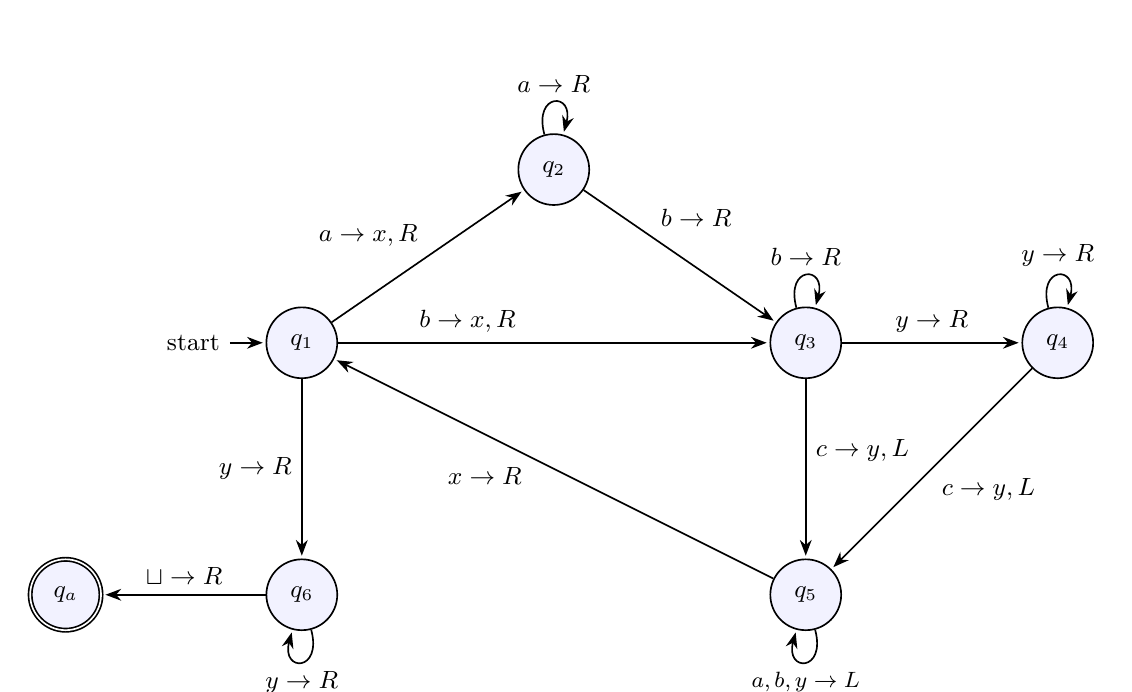
\begin{tikzpicture}[tm]
\node[state,initial] (q1) at (0,0) {$q_1$};
\node[state] (q2) at (3.2,2.2) {$q_2$};
\node[state] (q3) at (6.4,0) {$q_3$};
\node[state] (q4) at (9.6,0) {$q_4$};
\node[state] (q5) at (6.4,-3.2) {$q_5$};
\node[state] (q6) at (0,-3.2) {$q_6$};
\node[state,accepting] (qa) at (-3,-3.2) {$q_a$};
\path
 (q1) edge node {$a\to x,R$} (q2)
 (q1) edge node[pos=0.3] {$b\to x,R$} (q3)
 (q2) edge[loop above] node {$a\to R$} ()
 (q2) edge node[pos=0.35] {$b\to R$} (q3)
 (q3) edge[loop above] node {$b\to R$} ()
 (q3) edge node {$y\to R$} (q4)
 (q4) edge[loop above] node {$y\to R$} ()
 (q3) edge node[pos=0.4] {$c\to y,L$} (q5)
 (q4) edge node {$c\to y,L$} (q5)
 (q5) edge[loop below] node[lab] {$a,b,y\to L$} ()
 (q5) edge node[pos=0.55] {$x\to R$} (q1)
 (q1) edge[swap] node {$y\to R$} (q6)
 (q6) edge[loop below] node {$y\to R$} ()
 (q6) edge node[swap] {$\blank\to R$} (qa);
\end{tikzpicture}

{\footnotesize Missing transitions go to $q_{\mathrm{reject}}$.}
\end{center}

\begin{itemize}
\item $q_1$: leftmost unmatched symbol. $a$ or $b$: cross it. $y$: everything before the $c$'s is matched, go check the rest ($q_6$). $c$ or $\blank$: reject (a $c$ with no $a/b$ before it, or $n=m=0$).
\item $q_2$: inside the $a$-block; may only see $a$'s, then must see a $b$ (this enforces $m\ge1$).
\item $q_3$: inside the $b$-block; $b$'s, then either the first $c$ (cross it) or $y$'s ($q_4$).
\item $q_4$: skip already crossed $c$'s, cross the next $c$.
\item $q_5$: go back to the rightmost $x$. \quad $q_6$: accept iff only $y$'s remain.
\end{itemize}

\textbf{Why it decides $L$.} The states $q_2\to q_3\to q_4$ only allow the pattern $a^*\,b^+\,y^*\,c$, so every accepted string has the form $a^nb^mc^k$ with $m\ge1$; each round pairs one $a$/$b$ with one $c$, and $q_6$ accepts only if all $c$'s were used, so $k=n+m$. Conversely, every string of $L$ passes all these checks. Each round crosses two symbols, so the machine halts.

\textbf{Trace:} $abccc$: two rounds give $xxyyc$; $q_1$ reads $y$, $q_6$ reads $c$: reject (needs exactly $2$ $c$'s). $bacc$: $q_3$ reads $a$: reject.
\end{soln}

\begin{question}{6}
Give a high-level description of a Turing machine that decides $L=\{a^ib^jc^k\mid i,j,k\ge 0,\ k=ij\}$.
\end{question}
\begin{soln}
\textbf{Idea.} $ij$ is ``$j$ $c$'s for every $a$''. So for each $a$, sweep over the $b$'s and cross one $c$ per $b$.

$M=$ ``On input $w$:
\begin{enumerate}
\item Scan the input; if it is not of the form $a^*b^*c^*$, reject. Return to the left end.
\item For each $a$ (cross it off):
  \begin{enumerate}
  \item for each $b$: mark the $b$, and cross off one uncrossed $c$; if no uncrossed $c$ is left, \emph{reject};
  \item unmark all the $b$'s (so they can be used again for the next $a$).
  \end{enumerate}
\item When all $a$'s are crossed: if some $c$ is still uncrossed, \emph{reject}; otherwise \emph{accept}.''
\end{enumerate}

\textbf{Correctness.} Stage 2 crosses exactly $j$ $c$'s per $a$, hence $ij$ in total, rejecting as soon as there are fewer than needed. Stage 3 rejects if there are more. So the machine accepts iff $k=ij$. The cases $i=0$ or $j=0$ need no special treatment: nothing is crossed, and stage 3 accepts iff $k=0=ij$.

\textbf{Halting.} Stage 1 is one pass. Stage 2 runs $i$ outer and $j$ inner iterations, each a finite back-and-forth sweep. So the machine always halts.
\end{soln}

\begin{question}{7}
Consider the language $L=\{a^nb^{2n}\mid n>0\}$.
(a) Explain how a stack can be used to accept this language.
(b) Write a TM that simulates the stack behaviour to accept this language.
\end{question}
\begin{soln}
\textbf{(a) Stack idea (a PDA).} While reading $a$'s, \emph{push two} symbols $X$ for each $a$. While reading $b$'s, \emph{pop one} $X$ for each $b$. Accept iff the input ends exactly when the stack becomes empty, and there was at least one $a$. Then $\#b=2\cdot\#a$, and the $a$'s came first because once we start popping we never push again.

\textbf{(b) A 2-tape TM whose second tape is the stack.} Tape 1 holds the input (read left to right). Tape 2 is the stack: its head sits just right of the top symbol; a push writes $X$ and moves right, a pop moves left and erases. A transition label
\[
(s_1,s_2)\to(t_1,t_2),\,D_1D_2
\]
means: read $s_i$ on tape $i$, write $t_i$, move head $i$ in direction $D_i\in\{L,R,S\}$ ($S$ = stay).

\begin{center}
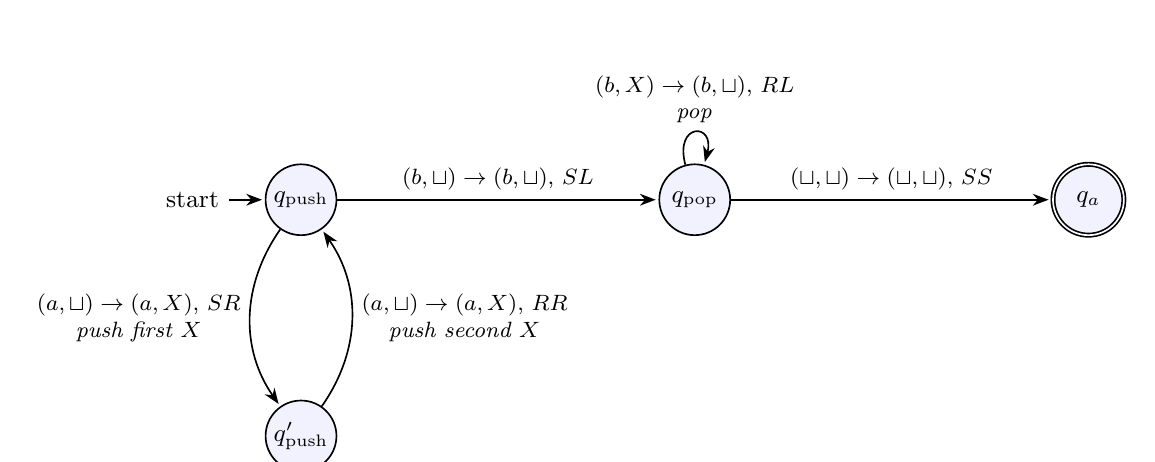
\begin{tikzpicture}[tm]
\node[state,initial] (p1) at (0,0) {$q_{\mathrm{push}}$};
\node[state] (p2) at (0,-3) {$q_{\mathrm{push}}'$};
\node[state] (pop) at (5,0) {$q_{\mathrm{pop}}$};
\node[state,accepting] (qa) at (10,0) {$q_a$};
\path
 (p1) edge[bend right=35,swap] node[lab] {$(a,\blank)\to(a,X),\,SR$\\ \emph{push first $X$}} (p2)
 (p2) edge[bend right=35,swap] node[lab] {$(a,\blank)\to(a,X),\,RR$\\ \emph{push second $X$}} (p1)
 (p1) edge node[lab] {$(b,\blank)\to(b,\blank),\,SL$} (pop)
 (pop) edge[loop above] node[lab] {$(b,X)\to(b,\blank),\,RL$\\ \emph{pop}} ()
 (pop) edge node[lab] {$(\blank,\blank)\to(\blank,\blank),\,SS$} (qa);
\end{tikzpicture}

{\footnotesize Missing transitions go to $q_{\mathrm{reject}}$.}
\end{center}

\begin{itemize}
\item $q_{\mathrm{push}}\leftrightarrow q'_{\mathrm{push}}$: each $a$ pushes two $X$'s (tape-1 head advances only after the second push).
\item On the first $b$, move the stack head onto the top $X$ and start popping.
\item $q_{\mathrm{pop}}$: each $b$ pops one $X$. Accept when the input ends and the stack is empty ($\blank$ on both tapes).
\end{itemize}

\textbf{Rejections:} an $a$ after a $b$ (no rule in $q_{\mathrm{pop}}$); a $b$ with empty stack, i.e. too many $b$'s ($(b,\blank)$ in $q_{\mathrm{pop}}$); input ending with a non-empty stack, i.e. too few $b$'s ($(\blank,X)$); and $n=0$ (blank in $q_{\mathrm{push}}$; a leading $b$ gives $(b,\blank)$ in $q_{\mathrm{pop}}$). Every step moves the input head right or moves the stack head, so the machine halts within $2|w|+2$ steps.

\textbf{Trace on $abb$:} push $X$, push $X$ (stack $XX$), read $b$: pop, $b$: pop, then $(\blank,\blank)$: accept. On $abbb$ the third $b$ meets an empty stack: reject.

(If a single tape is preferred: cross one $a$ and then two $b$'s per round; this is the same idea, with the uncrossed $b$'s playing the role of the stack.)
\end{soln}

\begin{question}{8}
Given binary representations of $x$ and $y$ as input to a Turing machine, describe how the machine would compute the following: (1) $x-1$ \quad (2) $x\times y$ \quad (3) $x^y$.
\end{question}
\begin{soln}
Numbers are written in binary, most significant bit first. For (2) and (3) the input is $x\#y$. We use a multitape TM (allowed, since it is equivalent to a single-tape TM by Q14).

\textbf{(1) $x-1$ (borrowing).} This is grade-school subtraction of 1:
\begin{enumerate}
\item Move to the last (least significant) bit.
\item While the bit is $0$: write $1$, move left (borrow).
\item At the first $1$: write $0$ and stop.
\item If the result starts with $0$ and has more than one bit, delete that leading $0$ (e.g.\ $1000-1=0111\to111$).
\end{enumerate}
Example: $10100-1$: the last two $0$'s become $1$'s and the $1$ becomes $0$, giving $10011$.
For $x=0$ we use the usual convention $0-1=0$ (check first whether all bits are $0$; if so leave the input unchanged).

\textbf{(2) $x\times y$ (shift and add, Horner's rule).} Tape 1: $x$; tape 2: $y$; tape 3: the running product $P$, initially $0$.
\[
\text{for each bit } b \text{ of } y \text{ from left to right:}\qquad
P\leftarrow 2P\ \ (\text{append a } 0),\qquad
\text{if } b=1:\ P\leftarrow P+x .
\]
The addition $P+x$ is done with both heads starting at the right ends, adding bit by bit right to left and keeping the carry in the finite control.
After the last bit $P=x\cdot y$, because $y=(\cdots((b_1)2+b_2)2+\cdots)2+b_k$.
Example: $x=101$ (5), $y=11$ (3): $P=0\to0+101=101\to1010+101=1111$ (15).

\textbf{(3) $x^y$ (square and multiply).} Tape for the result $R$, initially $1$:
\[
\text{for each bit } b \text{ of } y \text{ from left to right:}\qquad
R\leftarrow R\cdot R,\qquad
\text{if } b=1:\ R\leftarrow R\cdot x ,
\]
each multiplication using the subroutine from (2) (on extra work tapes).
This is the same Horner idea, with $+$ replaced by $\times$: if $y'$ is the prefix read so far, then $R=x^{y'}$, and reading a bit $b$ changes $y'$ to $2y'+b$, so $R$ becomes $x^{2y'+b}=(x^{y'})^2x^b$. In particular $x^0=1$ (the loop never multiplies by $x$).

\textbf{Halting.} Each loop runs once per bit of $y$ (finitely many), and each addition or multiplication halts. So all three machines halt with the answer on the tape.
\end{soln}

\begin{question}{9}
If TMs $M$, $M'$ compute $f(x)$, $g(x)$ for input $x$, construct a TM which can compute (1) $f(g(x))$, (2) $f^n(x)$ where $n$ is given as input.
\end{question}
\begin{soln}
``$M$ computes $f$'' means: started on $x$, $M$ halts with $f(x)$ on the tape. To run a machine as a \emph{subroutine} we simply copy its states and transitions into the new machine, and redirect its halting state to wherever we want to continue. Using two tapes keeps the bookkeeping simple (Q14).

\textbf{(1) $f\circ g$.}
$C=$ ``On input $x$:
\begin{enumerate}
\item Run $M'$ on $x$. It halts with $g(x)$ on the tape.
\item Move the head back to the left end, and run $M$ on $g(x)$. When it halts, the tape holds $f(g(x))$.''
\end{enumerate}
If $g(x)$ or $f(g(x))$ is undefined (the machine loops), so does $C$. In a single-tape version, $C$ marks the left end first so that it can find it again in step 2.

\textbf{(2) $f^n$, input $n\#x$ with $n$ in binary (or unary).}
Tape 1 holds the counter $n$, tape 2 holds the current value $v$.
$I=$ ``On input $n\#x$:
\begin{enumerate}
\item Copy $x$ to tape 2 and erase it from tape 1, leaving only $n$ there.
\item While $n\neq0$: run $M$ on tape 2 (replacing $v$ by $f(v)$); then decrement $n$ on tape 1 (Q8(1)).
\item Output tape 2.''
\end{enumerate}
\textbf{Invariant:} after $t$ iterations, tape 2 holds $f^t(x)$ and tape 1 holds $n-t$. So the loop runs exactly $n$ times and outputs $f^n(x)$ (for $n=0$ it outputs $x=f^0(x)$). If every call of $M$ halts, $I$ halts.
\end{soln}

\begin{question}{10}
(a) Design a Turing machine that takes as input two integers $m,n$ in unary and computes the quotient and the remainder when $m$ is divided by $n$.
(b) Hence (or otherwise) design a Turing machine that takes as input strings of the form $\{a^k\mid k>0\}$ and tests whether the input belongs to the language $\{a^{n!}\mid n>0\}$.
\end{question}
\begin{soln}
\textbf{(a) Division by repeated subtraction.} Input $1^m\#1^n$ with $n\ge1$ (if $n=0$, reject: division by $0$). Idea: subtract $n$ from $m$ as many times as possible. Each complete subtraction adds $1$ to the quotient; what is left at the end is the remainder.

The machine subtracts one unit at a time: it marks one $1$ of the divisor ($1\to y$) and crosses one $1$ of the dividend ($1\to x$). The quotient is built in unary to the right of a second $\#$.

$D=$ ``On input $1^m\#1^n$:
\begin{enumerate}
\item Write $\#$ after the input (tape: $1^m\#1^n\#$).
\item \emph{One unit:} find the leftmost unmarked $1$ of the divisor.
  \begin{itemize}
  \item If there is none (all $n$ are marked $y$): one full copy of $n$ has been subtracted. Append a $1$ to the quotient at the right end, unmark all divisor symbols ($y\to1$), and repeat stage 2.
  \item Otherwise, look for an uncrossed $1$ in the dividend. If there is one, cross it ($1\to x$), mark this divisor $1$ as $y$, and repeat stage 2. If there is none, go to stage 3.
  \end{itemize}
\item \emph{Done:} the dividend is used up in the middle of a round. The remainder $r$ is the number of $y$'s, the quotient $q$ is the number of $1$'s after the second $\#$. Rewrite the tape as $1^q\#1^r$ and halt.''
\end{enumerate}

\textbf{Correctness.} Every crossed dividend $1$ is paired with exactly one marked divisor $1$, so when the machine stops $m=q\cdot n+r$, where $r$ is the number of $y$'s. We have $r<n$, because a round in which all $n$ divisor symbols are marked is counted in $q$ and reset. So $q=\lfloor m/n\rfloor$ and $r=m\bmod n$.
\textbf{Halting.} Every pass of stage 2 either crosses a new dividend $1$ (at most $m$ times) or is one of the at most $q+1$ round resets, so stage 3 is always reached.
Example: $m=7,n=3$: two full rounds ($q=2$), then one more $1$ is crossed and the dividend is empty, so $r=1$: output $11\#1$.

\textbf{(b) Testing $k=n!$ by dividing by $2,3,4,\dots$} Use $D$ from (a) as a subroutine.

$F=$ ``On input $a^k$ ($k>0$):
\begin{enumerate}
\item Let $v=k$ (rewrite the $a$'s as $1$'s) and $d=2$ (written $11$ on a second tape).
\item If $v=1$, \emph{accept}.
\item Divide $v$ by $d$ using $D$. If the remainder is not $0$, \emph{reject}.
\item Let $v\leftarrow$ quotient, $d\leftarrow d+1$ (append a $1$), and go to stage 2.''
\end{enumerate}

\textbf{Correctness.} When stage 2 is reached for the $j$-th time ($j\ge1$), $v=k/j!$, since we have divided by $2,3,\dots,j$ in turn.
\begin{itemize}
\item If $k=n!$: every division up to $d=n$ is exact, and after it $v=n!/n!=1$, so $F$ accepts. (It cannot reject earlier: $j!$ divides $n!$ for $j\le n$.)
\item If $F$ accepts at the $j$-th visit of stage 2, then $1=v=k/j!$, i.e.\ $k=j!$ with $j\ge1$.
\end{itemize}
So $F$ accepts exactly $\{a^{n!}\mid n>0\}$. Note that $k=1=1!$ is accepted immediately.

\textbf{Halting.} Every exact division by $d\ge2$ at least halves $v$, and $v\ge1$. So after at most $\log_2 k$ rounds, $F$ either accepts ($v=1$) or rejects (a nonzero remainder; this includes the case $1<v<d$, where $q=0$ and $r=v$).
Examples: $k=6$: $6/2=3$, $3/3=1$, accept. $k=4$: $4/2=2$, then $2/3$ leaves remainder $2$, reject.
\end{soln}

\begin{question}{11}
Describe a Turing machine that decides whether all symbols in an input string are distinct. Assume the input alphabet is finite. Explain why the machine always halts.
\end{question}
\begin{soln}
\textbf{Idea.} Take the symbols one at a time as a ``pivot'' and check that the pivot does not occur again to its right. Since $\Sigma$ is finite, the machine can \emph{remember the pivot symbol in its state} (one copy of the scanning states for each $\sigma\in\Sigma$).

$M=$ ``On input $w$:
\begin{enumerate}
\item Mark the left end (replace the first symbol $a$ by a special version $\hat a$, which still counts as the symbol $a$), so the machine can find it again.
\item Find the leftmost unmarked symbol $\sigma$. If there is none, \emph{accept}. Otherwise mark it as $\dot\sigma$ and remember $\sigma$ in the state.
\item Scan right to the end of the input. If an unmarked $\sigma$ is seen, \emph{reject}.
\item Return to the left end and go to stage 2.''
\end{enumerate}

\textbf{Correctness.} If $w_i=w_j$ with $i<j$, then when $w_i$ is the pivot, stage 3 sees $w_j$ and rejects. If all symbols are distinct, no scan ever rejects, and after $|w|$ rounds everything is marked: accept.

\textbf{Halting.} Every round marks one more cell, so there are at most $|w|+1$ rounds, and each round is one sweep right and one sweep back over $|w|$ cells (at most $O(|w|^2)$ steps in total). Finiteness of $\Sigma$ is what makes ``remember $\sigma$'' possible with finitely many states.

(Shortcut: if $|w|>|\Sigma|$ the answer is ``no'' by the pigeonhole principle, but the machine above does not need this.)
\end{soln}

\begin{question}{12}
Explain the difference between a Turing machine that recognizes a language and one that decides a language.
\end{question}
\begin{soln}
On an input, a TM can \emph{accept}, \emph{reject}, or \emph{loop} (run forever).
\begin{itemize}
\item $M$ \textbf{recognizes} $L$ if $L=L(M)=\{w\mid M\text{ accepts }w\}$. On $w\notin L$ it may reject \emph{or loop}.
\item $M$ \textbf{decides} $L$ if it recognizes $L$ \emph{and halts on every input}: it accepts every $w\in L$ and rejects every $w\notin L$.
\end{itemize}
So a recognizer gives a guaranteed ``yes'' answer, but for a ``no'' you may wait forever without learning anything. A decider always answers.

Every decider is a recognizer, so decidable $\subseteq$ Turing-recognizable. The inclusion is strict: $\Atm=\{\enc{M,w}\mid M \text{ accepts } w\}$ is recognized by the universal TM (simulate $M$ on $w$), which loops when $M$ loops, and no TM decides $\Atm$ (Sipser Thm 4.11).
A useful fact: $L$ is decidable $\iff$ both $L$ and $\comp L$ are Turing-recognizable (Thm 4.22).
\end{soln}

\begin{question}{13}
Explain why allowing a Turing machine's head to stay in place during a transition does not increase its computational power. Describe how such a transition can be simulated by a standard Turing machine.
\end{question}
\begin{soln}
A ``stay'' model has $\delta:Q\times\Gamma\to Q\times\Gamma\times\{L,R,S\}$.

\textbf{Simulation.} Replace each stay move $\delta(q,a)=(r,b,S)$ by two ordinary moves through a new state $p$:
\[
\delta(q,a)=(p,\,b,\,R),\qquad \delta(p,c)=(r,\,c,\,L)\quad\text{for every }c\in\Gamma .
\]
That is: write $b$ and step right, then step back left without changing anything. The result is the same configuration (cell is $b$, head on the same cell, state $r$), reached in two steps instead of one. All $L/R$ moves are copied unchanged.

\emph{Why right-then-left?} The tape has a left end, and a left move from the leftmost cell does not move the head. A right move always moves, so ``right then left'' always returns to the same cell.

\textbf{No extra power.} Each step of the stay-machine becomes one or two steps of the standard machine, so both accept, reject and loop on exactly the same inputs. Conversely, a standard TM is a stay-TM that never uses $S$. Hence both models recognize (and decide) the same languages.
\end{soln}

\begin{question}{14}
Show that every multitape Turing machine can be simulated by a single-tape Turing machine. Explain the representation of the multiple tapes and head positions on the single tape.
\end{question}
\begin{soln}
(Sipser Thm 3.13.) Let $M$ have $k$ tapes. We build a single-tape TM $S$.

\textbf{Representation.} Write the contents of the $k$ tapes one after another, separated by $\#$. Mark each head position by putting a \emph{dot} on the symbol under that head; so for every $a\in\Gamma$ the tape alphabet of $S$ contains both $a$ and $\dot a$, plus $\#$:
\[
\#\;\underbrace{\cdots\dot a\cdots}_{\text{tape 1}}\;\#\;\underbrace{\cdots\dot b\cdots}_{\text{tape 2}}\;\#\;\cdots\;\#\;\underbrace{\cdots\dot c\cdots}_{\text{tape }k}\;\#
\]

\begin{center}
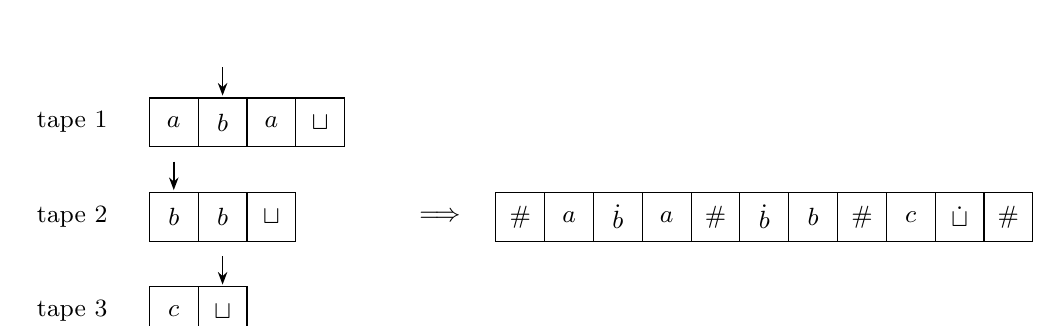
\begin{tikzpicture}[cell/.style={draw,minimum width=0.62cm,minimum height=0.62cm,inner sep=0pt,font=\small},
  hd/.style={-{Stealth[length=1.6mm]},semithick}]
  \foreach \t/\y/\cont in {1/0/{a,b,a},2/-1.2/{b,b},3/-2.4/{c}}{
    \node[anchor=east,font=\small] at (-0.1,\y) {tape \t};
    \foreach \s [count=\i] in \cont {\node[cell] at (0.62*\i,\y) {$\s$};}
  }
  \node[cell] at (2.48,0) {$\blank$};
  \node[cell] at (1.86,-1.2) {$\blank$};
  \node[cell] at (1.24,-2.4) {$\blank$};
  \draw[hd] (1.24,0.7) -- (1.24,0.34);
  \draw[hd] (0.62,-0.5) -- (0.62,-0.86);
  \draw[hd] (1.24,-1.7) -- (1.24,-2.06);
  \node[font=\small] at (4.0,-1.2) {$\Longrightarrow$};
  \foreach \s [count=\i] in {\#,a,\dot b,a,\#,\dot b,b,\#,c,\dot\blank,\#}{
    \node[cell] at (4.4+0.62*\i,-1.2) {$\s$};}
\end{tikzpicture}

{\footnotesize Three tapes (arrows = heads) and the single tape of $S$. Tape 3's head is on the blank just after $c$, so that blank is written explicitly.}
\end{center}

\textbf{Simulating one step of $M$.}
\begin{enumerate}
\item \emph{Read:} sweep from the left $\#$ to the right end, and remember the $k$ dotted symbols in the finite control (finitely many possibilities, since $k$ and $\Gamma$ are fixed).
\item \emph{Update:} now $\delta_M$ tells $S$ the new state, the $k$ symbols to write and the $k$ moves. Sweep again; at each dotted symbol write the new symbol and move the dot one cell left or right (or keep it in place).
\item \emph{Growing a tape:} if a dot moves right onto a $\#$, that virtual head has reached unused blank space on its tape. $S$ writes a dotted blank $\dot\blank$ there and shifts everything from this cell onwards one cell to the right. If a dot would move left past a $\#$, it stays where it is (left end of that tape).
\end{enumerate}
Initially $S$ rewrites its input $w=w_1\cdots w_n$ as $\#\dot w_1w_2\cdots w_n\#\dot\blank\#\cdots\#\dot\blank\#$, which represents $M$'s start configuration.

\textbf{Correctness.} After each simulated step, the tape of $S$ represents exactly the $k$ tapes and head positions of $M$, and the state of $S$ records $M$'s state. $S$ accepts/rejects when $M$ does, and loops when $M$ loops, so $L(S)=L(M)$ (and $S$ is a decider if $M$ is). Conversely, a single-tape TM is a 1-tape multitape TM. So the two models are equivalent.
\end{soln}

\begin{question}{15}
A multi-head Turing machine is a single-tape Turing machine with multiple heads operating on the same tape. Show that multi-head Turing machines are equivalent in computational power to standard single-head Turing machines.
\end{question}
\begin{soln}
A $k$-head TM has $\delta:Q\times\Gamma^k\to Q\times\Gamma^k\times\{L,R\}^k$: all heads read, write and move in one step. (If two heads on the same cell write different symbols, fix a rule, e.g.\ the head with the larger number wins.)

\textbf{Single-head $\Rightarrow$ multi-head:} trivial; use only head 1.

\textbf{Multi-head $\Rightarrow$ single-head.} The idea is the same as in Q14, except that now all heads share \emph{one} tape, so no separators are needed: just mark which heads are on each cell. The simulator $S$ uses the symbols
\[
(a,H),\qquad a\in\Gamma,\ H\subseteq\{1,\dots,k\}\quad(\text{the heads standing on this cell}),
\]
which is a finite alphabet ($|\Gamma|\cdot 2^k$ symbols).

\begin{center}
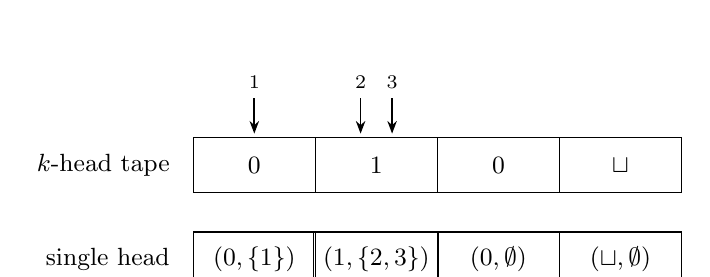
\begin{tikzpicture}[cell/.style={draw,minimum width=1.55cm,minimum height=0.7cm,font=\small},
  hd/.style={-{Stealth[length=1.6mm]},semithick}]
  \node[anchor=east,font=\small] at (0.4,0) {$k$-head tape};
  \foreach \s [count=\i] in {0,1,0,\blank}{\node[cell] at (1.55*\i-0.2,0) {$\s$};}
  \draw[hd] (1.35,0.85) node[above,font=\scriptsize]{1} -- (1.35,0.4);
  \draw[hd] (2.7,0.85) node[above,font=\scriptsize]{2} -- (2.7,0.4);
  \draw[hd] (3.1,0.85) node[above,font=\scriptsize]{3} -- (3.1,0.4);
  \node[anchor=east,font=\small] at (0.4,-1.2) {single head};
  \foreach \s [count=\i] in {{(0,\{1\})},{(1,\{2,3\})},{(0,\emptyset)},{(\blank,\emptyset)}}{\node[cell] at (1.55*\i-0.2,-1.2) {$\s$};}
\end{tikzpicture}

{\footnotesize Heads 2 and 3 share a cell; the set $H$ records them.}
\end{center}

Initially $S$ puts $\{1,\dots,k\}$ on the first cell (all heads start there) and $\emptyset$ on the other cells.
One step of the $k$-head machine is simulated by:
\begin{enumerate}
\item \emph{Read:} sweep the used part of the tape; for each $i$ remember the symbol $a_i$ in the cell whose set contains $i$.
\item \emph{Write:} apply $\delta$ to get the new state, the symbols $b_i$ and the moves $D_i$. Sweep again and write the new symbols in the cells that carry heads.
\item \emph{Move:} for each $i$, remove $i$ from its cell's set and add it to the set of the left or right neighbour (if the head is on the leftmost cell and moves left, it stays put; if it moves right onto fresh tape, write $(\blank,\{i\})$ there).
\end{enumerate}
After each round the tape of $S$ represents the tape and all head positions, so $S$ accepts/rejects/loops exactly when the $k$-head machine does. Hence the models are equivalent.
\end{soln}

\begin{question}{16}
Show that every non-deterministic Turing machine can be simulated by a deterministic Turing machine. Explain how the deterministic machine explores the computation branches.
\end{question}
\begin{soln}
(Sipser Thm 3.16.) The computation of an NTM $N$ on $w$ is a \textbf{tree}: the root is the start configuration, and the children of a node are the configurations reachable in one step. $N$ accepts $w$ iff \emph{some} node of the tree is accepting. Each node has at most $b$ children, where $b$ is the largest number of choices in $\delta_N$.

\textbf{Key idea: search the tree breadth-first.} Depth-first search is wrong, since it can go down an infinite branch and never come back, even if an accepting node exists elsewhere. Breadth-first search reaches every node at depth $d$ after finitely many steps.

\textbf{Addresses.} A node is named by its \emph{address}: the string of choices leading to it from the root (choice $\in\{1,\dots,b\}$). Listing all strings over $\{1,\dots,b\}$ in order of length, i.e.\ $\eps,1,2,\dots,b,11,12,\dots$, visits the tree level by level.

\begin{center}
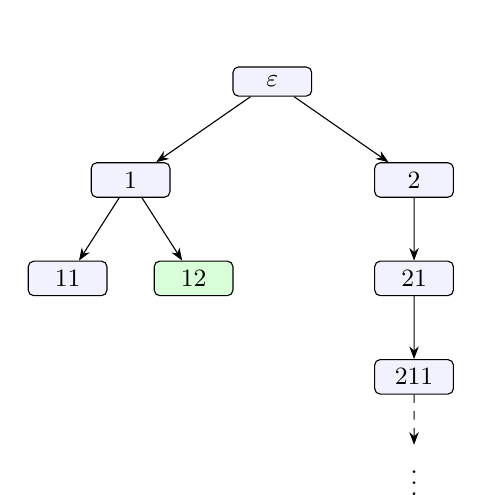
\begin{tikzpicture}[nd/.style={draw,rounded corners=2pt,minimum width=1.0cm,font=\small,fill=blue!5},
  level distance=1.25cm,
  level 1/.style={sibling distance=3.6cm},level 2/.style={sibling distance=1.6cm},
  edge from parent/.style={draw,-{Stealth[length=1.6mm]}}]
  \node[nd] {$\eps$}
    child {node[nd] {$1$}
      child {node[nd] {$11$}}
      child {node[nd,fill=green!15] {$12$}}}
    child {node[nd] {$2$}
      child {node[nd] {$21$}
        child {node[nd] {$211$}
          child {node[font=\small] {$\vdots$} edge from parent[dashed]}}}};
\end{tikzpicture}

{\footnotesize Here $b=2$. Branch $2,21,211,\dots$ is infinite; depth-first search could follow it forever. Breadth-first order $\eps,1,2,11,12,\ldots$ reaches the accepting node $12$ (green) after five addresses.}
\end{center}

\textbf{The deterministic 3-tape machine $D$.}
\begin{itemize}
\item Tape 1: the input $w$ (never changed).
\item Tape 2: the tape of $N$ on the branch currently being simulated.
\item Tape 3: the current address.
\end{itemize}
$D=$ ``\begin{enumerate}
\item Start with address $\eps$ on tape 3.
\item Copy $w$ to tape 2. Simulate $N$, using the symbols of tape 3 one by one as the choices. Stop the simulation when the address runs out, when a choice is invalid, or when $N$ rejects. If $N$ accepts, \emph{accept}.
\item Replace tape 3 by the next address in the order above and go to stage 2.''
\end{enumerate}

\textbf{Correctness.} If $N$ accepts $w$, some accepting node has a finite address $\alpha$. Only finitely many addresses come before $\alpha$, and each simulation is finite, so $D$ reaches $\alpha$ and accepts. If $N$ does not accept, $D$ never accepts. So $L(D)=L(N)$, and by Q14 $D$ can be made single-tape.

\textbf{If $N$ is a decider} (all branches halt on all inputs), the tree is finite (König's lemma: a finitely-branching tree with no infinite branch is finite). Modify $D$ to \emph{reject} when it finds a depth $d$ at which every branch has already halted without accepting. Then $D$ is a decider too.
\end{soln}

\begin{question}{17}
Describe a Turing machine that, given an encoding of an undirected graph $G=(V,E)$ followed by two vertices $s,t\in V$, decides whether a path exists between $s$ and $t$. You may assume the input lists the vertices first, followed by the edges and then $s,t$. Explain why the machine halts on every valid input.
\end{question}
\begin{soln}
\textbf{Idea.} Spread marks from $s$ along edges (``flood fill'') until nothing new gets marked; then check whether $t$ got marked.

$M=$ ``On input $\enc{G,s,t}$:
\begin{enumerate}
\item Check the input is a valid encoding (vertex list, edge list with endpoints in $V$, and $s,t\in V$); if not, \emph{reject}.
\item Mark $s$.
\item Repeat until no new vertex is marked:\\
\hspace*{1.5em}scan all edges; for each edge $\{u,v\}$ with exactly one endpoint marked, mark the other.
\item If $t$ is marked, \emph{accept}; otherwise \emph{reject}.''
\end{enumerate}

\begin{center}
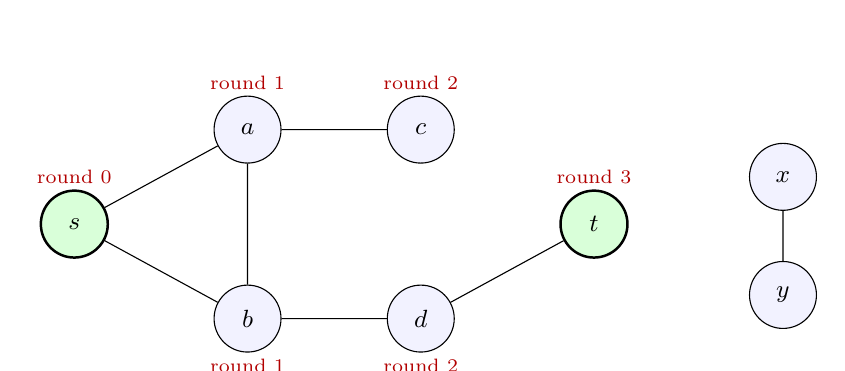
\begin{tikzpicture}[v/.style={circle,draw,minimum size=8.5mm,inner sep=0pt,font=\small,fill=blue!5},
  tt/.style={v,fill=green!15,line width=0.9pt}]
  \node[tt] (s) at (0,0) {$s$};
  \node[v] (a) at (2.2,1.2) {$a$};
  \node[v] (b) at (2.2,-1.2) {$b$};
  \node[v] (c) at (4.4,1.2) {$c$};
  \node[v] (d) at (4.4,-1.2) {$d$};
  \node[tt] (t) at (6.6,0) {$t$};
  \node[v] (x) at (9,0.6) {$x$};
  \node[v] (y) at (9,-0.9) {$y$};
  \draw (s)--(a) (s)--(b) (a)--(c) (b)--(d) (d)--(t) (a)--(b) (x)--(y);
  \foreach \n/\r/\dy in {s/0/6,a/1/6,b/1/-6,c/2/6,d/2/-6,t/3/6}{\node[font=\scriptsize,text=red!70!black] at ([yshift=\dy mm]\n) {round \r};}
\end{tikzpicture}

{\footnotesize Marking rounds starting from $s$: $t$ is marked in round 3, so the machine accepts. $x$ and $y$ are never marked (another component).}
\end{center}

\textbf{Correctness.} By induction, after round $i$ the marked vertices are exactly those at distance $\le i$ from $s$. So when no new vertex is marked, the marked vertices are exactly those reachable from $s$, and $t$ is marked iff an $s$--$t$ path exists.

\textbf{Halting.} Each round except the last marks at least one new vertex, so there are at most $|V|$ rounds, and each round is a finite scan of the edge list. Hence $M$ always halts (in time polynomial in the input length).
\end{soln}

\begin{question}{18}
Describe a Turing machine that, given an encoding of an undirected graph $G=(V,E)$, decides whether the graph contains a cycle. You may assume the input lists the vertices first, followed by the edges. Explain why the machine halts on every valid input.
\end{question}
\begin{soln}
\textbf{Key fact.} An edge $\{u,v\}$ lies on a cycle $\iff$ $u$ and $v$ are still connected after deleting that edge. (The rest of the cycle is a second route from $u$ to $v$.)

Deleting the edge is what prevents the false ``cycle'' $u\to v\to u$ that walks along the same edge and back.

\begin{center}
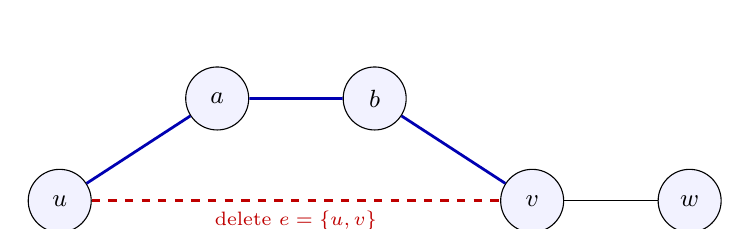
\begin{tikzpicture}[v/.style={circle,draw,minimum size=8mm,inner sep=0pt,font=\small,fill=blue!5}]
  \node[v] (u) at (0,0) {$u$};
  \node[v] (a) at (2,1.3) {$a$};
  \node[v] (b) at (4,1.3) {$b$};
  \node[v] (v) at (6,0) {$v$};
  \node[v] (w) at (8,0) {$w$};
  \draw[line width=1pt,blue!70!black] (u)--(a)--(b)--(v);
  \draw[line width=1pt,red!75!black,dashed] (u)--node[below,font=\scriptsize]{delete $e=\{u,v\}$} (v);
  \draw (v)--(w);
\end{tikzpicture}

{\footnotesize After deleting $e$, $u$ and $v$ are still connected (blue path), so $e$ is on the cycle $u,a,b,v,u$. For $e'=\{v,w\}$, deleting it disconnects $v$ from $w$, so $e'$ is on no cycle.}
\end{center}

$C=$ ``On input $\enc{G}$:
\begin{enumerate}
\item Check the encoding; if invalid, \emph{reject}.
\item For each edge $e=\{u,v\}$ in the list:\\
\hspace*{1.5em}run the path decider $M$ of Q17 on $\enc{G-e,\,u,\,v}$; if it accepts, \emph{accept}.
\item \emph{Reject}.''
\end{enumerate}
(If self-loops $\{u,u\}$ or repeated edges are allowed in the encoding, they form cycles: accept them directly in stage 1.)

\textbf{Correctness.} If $G$ has a cycle, then for any edge $e=\{u,v\}$ on it, the rest of the cycle is a $u$--$v$ path in $G-e$, so stage 2 accepts. Conversely, if $G-e$ has a $u$--$v$ path $P$, then $P$ followed by $e$ is a cycle in $G$ (in a simple graph $P$ has length $\ge2$, as $e$ was removed).

\textbf{Halting.} Stage 2 makes $|E|$ calls to $M$, and $M$ always halts (Q17). So $C$ always halts.

\emph{Alternative:} $G$ is acyclic (a forest) $\iff |E|=|V|-c$, where $c$ is the number of connected components; so $G$ has a cycle $\iff |E|>|V|-c$. Counting components with the marking procedure of Q17 gives another decider.
\end{soln}

\begin{question}{19}
Consider the problem of determining whether a given DFA accepts at least one string. Describe an algorithm for solving this problem and explain why it always terminates.
\end{question}
\begin{soln}
The language is $\{\enc{A}\mid A \text{ is a DFA and } L(A)\neq\emptyset\}$.

\textbf{Key fact.} $A$ accepts some string $\iff$ some accept state can be reached from the start state by following transitions (the labels along the path spell an accepted string). So this is just graph reachability on the state diagram.

$T=$ ``On input $\enc{A}$, $A=(Q,\Sigma,\delta,q_0,F)$:
\begin{enumerate}
\item Mark $q_0$.
\item Repeat until no new state is marked: mark every state $\delta(p,a)$ with $p$ marked and $a\in\Sigma$.
\item If some state of $F$ is marked, \emph{accept}; otherwise \emph{reject}.''
\end{enumerate}
(This is Sipser's $E_{\mathrm{DFA}}$ decider, Thm 4.4, with accept and reject swapped.)

\textbf{Termination.} Each round except the last marks a new state, and there are only $|Q|$ states, so there are at most $|Q|$ rounds, each finite. Note that we never try strings one by one; $L(A)$ may be infinite, but the state graph is finite.
\end{soln}

\begin{question}{20}
For the following language, determine whether it is decidable or undecidable:
$T=\{\enc{G,H}\mid G,H \text{ are CFGs where } L(G)\cap L(H)\neq\emptyset\}$.
\end{question}
\begin{soln}
\textbf{$T$ is undecidable} (though it is Turing-recognizable).

\textbf{Why the obvious approach fails.} CFLs are \emph{not} closed under intersection, so we cannot build a CFG for $L(G)\cap L(H)$ and test emptiness (as we did for DFAs).

\textbf{Proof: reduce PCP to $T$.} Recall (Sipser Thm 5.15) that PCP is undecidable: given dominoes $\bigl[\tfrac{t_1}{b_1}\bigr],\dots,\bigl[\tfrac{t_k}{b_k}\bigr]$, is there a sequence $i_1,\dots,i_m$ ($m\ge1$) with $t_{i_1}\cdots t_{i_m}=b_{i_1}\cdots b_{i_m}$?

Given an instance $P$, take new symbols $a_1,\dots,a_k$ (one ``index'' symbol per domino) and build two grammars:
\[
G_{\mathrm{top}}:\ S\to t_i\,S\,a_i \;\mid\; t_i\,a_i,
\qquad\qquad
G_{\mathrm{bot}}:\ S\to b_i\,S\,a_i \;\mid\; b_i\,a_i
\qquad(i=1,\dots,k).
\]
Then
\[
L(G_{\mathrm{top}})=\{\,t_{i_1}\cdots t_{i_m}\,a_{i_m}\cdots a_{i_1}\,\},\qquad
L(G_{\mathrm{bot}})=\{\,b_{i_1}\cdots b_{i_m}\,a_{i_m}\cdots a_{i_1}\,\}.
\]
The suffix $a_{i_m}\cdots a_{i_1}$ records which dominoes were used.

\textbf{Claim:} $P$ has a match $\iff L(G_{\mathrm{top}})\cap L(G_{\mathrm{bot}})\neq\emptyset$.
\begin{itemize}
\item[($\Rightarrow$)] If $i_1,\dots,i_m$ is a match, then the string $t_{i_1}\cdots t_{i_m}a_{i_m}\cdots a_{i_1}=b_{i_1}\cdots b_{i_m}a_{i_m}\cdots a_{i_1}$ is in both languages.
\item[($\Leftarrow$)] Suppose a string $z$ is in both. The $a$'s do not occur in any $t_i,b_i$, so the index suffix of $z$ is the same in both derivations. Hence both used the same sequence $i_1,\dots,i_m$, and removing the suffix gives $t_{i_1}\cdots t_{i_m}=b_{i_1}\cdots b_{i_m}$: a match.
\end{itemize}
The map $P\mapsto\enc{G_{\mathrm{top}},G_{\mathrm{bot}}}$ is computable, so $\mathrm{PCP}\redm T$. If $T$ were decidable, PCP would be decidable. Contradiction. Hence $T$ is undecidable.

\textbf{$T$ is recognizable:} try strings $z=\eps,0,1,00,\ldots$ in order, and use the $A_{\mathrm{CFG}}$ decider (Thm 4.7) to test $z\in L(G)$ and $z\in L(H)$. Accept if both hold. So $\comp T$ (``the intersection is empty'') is not even recognizable (otherwise $T$ would be decidable by Thm 4.22).
\end{soln}

\begin{question}{21}
Show that the language
\[L_1=\{w\in\{0,1\}^*\mid w \text{ is a binary representation of } 2^n \text{ for some } n\ge 0\}\]
is decidable.
\end{question}
\begin{soln}
In binary, $2^n$ is a $1$ followed by $n$ zeros ($1,10,100,\dots$). With the usual convention of no leading zeros,
\[
L_1=\{1,10,100,1000,\dots\}=L(10^*),
\]
which is \textbf{regular}. Every regular language is decidable: simulate its DFA (Sipser Thm 4.1).

\begin{center}
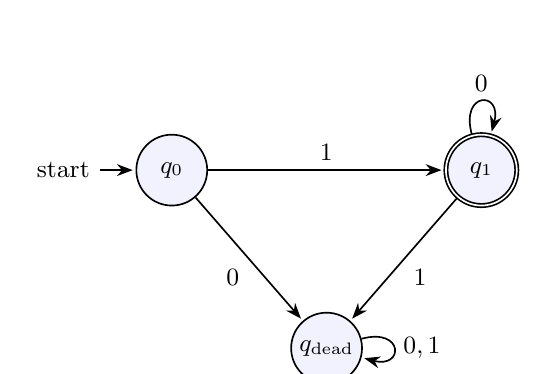
\begin{tikzpicture}[tm,node distance=3cm]
\node[state,initial] (q0) {$q_0$};
\node[state,accepting,right=of q0] (q1) {$q_1$};
\node[state,below=1.8cm of $(q0)!0.5!(q1)$] (d) {$q_{\mathrm{dead}}$};
\path
 (q0) edge node {$1$} (q1)
 (q1) edge[loop above] node {$0$} ()
 (q0) edge[swap] node {$0$} (d)
 (q1) edge node {$1$} (d)
 (d) edge[loop right] node {$0,1$} ();
\end{tikzpicture}
\end{center}

Decider: ``On input $w$: run this DFA on $w$; accept iff it ends in $q_1$.'' It halts after $|w|$ steps.
(If leading zeros are allowed, $L_1=L(0^*10^*)$, again regular, so the answer does not change.)
\end{soln}

\begin{question}{22}
Show that the language
\[L_2=\{\enc{M}\mid M \text{ is a DFA that accepts } w^R \text{ whenever it accepts } w\}\]
is decidable, where $w^R$ denotes the reverse of $w$.
\end{question}
\begin{soln}
Let $L=L(M)$. The condition says $L\subseteq L^R$.

\textbf{Step 1: the condition means $L=L^R$.} If $L\subseteq L^R$, reverse both sides: $L^R\subseteq (L^R)^R=L$. So $L=L^R$.

\textbf{Step 2: a DFA for $L^R$.} Reverse every arrow of $M$, make the old start state the only accept state, and add a new start state with $\eps$-moves to all old accept states. This NFA $N$ reads a string backwards along a path of $M$, so $L(N)=L^R$. Convert $N$ to a DFA $M^R$ by the subset construction.

\begin{center}
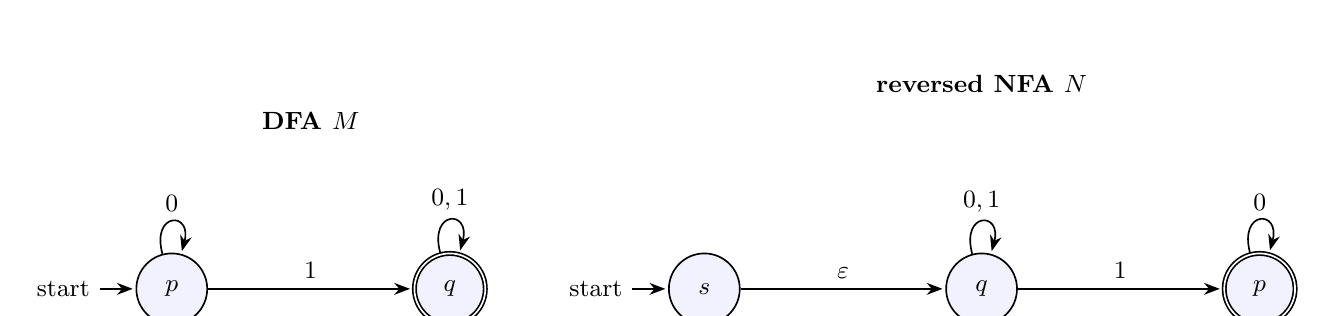
\begin{tikzpicture}[tm,node distance=2.6cm]
\node[state,initial] (p) {$p$};
\node[state,accepting,right=of p] (q) {$q$};
\path (p) edge node {$1$} (q)
      (p) edge[loop above] node {$0$} ()
      (q) edge[loop above] node {$0,1$} ();
\node[above=1.9cm of $(p)!0.5!(q)$,font=\bfseries\small] {DFA $M$};
\node[state,initial,right=2.3cm of q] (s) {$s$};
\node[state,right=of s] (q2) {$q$};
\node[state,accepting,right=of q2] (p2) {$p$};
\path (s) edge node {$\eps$} (q2)
      (q2) edge node {$1$} (p2)
      (q2) edge[loop above] node {$0,1$} ()
      (p2) edge[loop above] node {$0$} ();
\node[above=1.9cm of q2,font=\bfseries\small] {reversed NFA $N$};
\end{tikzpicture}

{\footnotesize $M$ accepts strings containing a $1$; so does $N$ (this $L$ happens to satisfy $L=L^R$).}
\end{center}

\textbf{Step 3: decide.}
$T=$ ``On input $\enc{M}$: build $M^R$ as above; run the $\mathit{EQ}_{\mathrm{DFA}}$ decider (Thm 4.5) on $\enc{M,M^R}$; accept iff it accepts.''
Every step is a finite construction or a decider, so $T$ halts, and it accepts iff $L(M)=L(M)^R$, i.e.\ iff $\enc M\in L_2$.
\end{soln}

\begin{question}{23}
For languages $L_1,L_2$, define $L_1\oplus L_2=\{w\mid (w\in L_1 \text{ and } w\notin L_2) \text{ or } (w\notin L_1 \text{ and } w\in L_2)\}$. True or false: if $L_1$ and $L_2$ are decidable, then $L_1\oplus L_2$ is decidable. Justify.
\end{question}
\begin{soln}
\textbf{True.} Let $M_1,M_2$ decide $L_1,L_2$.

$M=$ ``On input $w$: run $M_1$ on $w$ and run $M_2$ on $w$ (both halt). Accept iff exactly one of them accepted.''

$M$ always halts because $M_1$ and $M_2$ do, and it accepts exactly the strings in exactly one of $L_1,L_2$, i.e.\ $L_1\oplus L_2$.
(Equivalently, $L_1\oplus L_2=(L_1\cap\comp{L_2})\cup(\comp{L_1}\cap L_2)$, and decidable languages are closed under $\cap,\cup$ and complement.)
\end{soln}

\begin{question}{24}
Let $A$ be a language that is Turing-recognizable but not decidable. Is the language $\comp A$ Turing-recognizable? Is $\comp A$ Turing-decidable? Justify your answers.
\end{question}
\begin{soln}
\textbf{$\comp A$ is not Turing-recognizable.} Recall Thm 4.22: a language is decidable iff both it and its complement are recognizable. (Run the two recognizers in parallel; on every input exactly one of them accepts.) If $\comp A$ were recognizable, then $A$ and $\comp A$ would both be recognizable, so $A$ would be decidable, which is a contradiction.

\textbf{$\comp A$ is not decidable.} Every decidable language is recognizable, and $\comp A$ is not recognizable. (Alternatively: if $\comp A$ were decidable, then so would be $A=\comp{\comp A}$, by swapping accept and reject.)

Example: $A=\Atm$; $\comp{\Atm}$ is not recognizable (Cor 4.23).
\end{soln}

\begin{question}{25}
True or false: all unary languages $L\subseteq\{1\}^*$ are Turing-recognizable. Justify.
\end{question}
\begin{soln}
\textbf{False.}

\textbf{Counting argument.} There are only countably many TMs (Q2), so only countably many recognizable languages. But the unary languages are all subsets of the countably infinite set $\{1\}^*=\{\eps,1,11,\dots\}$, and there are uncountably many such subsets (as many as subsets of $\mathbb N$, by Cantor). So some unary language is not recognized by any TM.

\textbf{An explicit one (diagonalization).} List all TMs as $M_0,M_1,M_2,\dots$ and let
\[
D=\{1^i\mid M_i \text{ does not accept } 1^i\}.
\]
If some $M_j$ recognized $D$, then $1^j\in D\iff M_j$ does not accept $1^j\iff 1^j\notin L(M_j)=D$, which is a contradiction. So $D$ is a unary language that is not Turing-recognizable.
\end{soln}

\begin{question}{26}
Show that the language
\[L_3=\{\enc M\mid M \text{ is a DFA that accepts some string with more 1's than 0's}\}\]
is decidable.
\end{question}
\begin{soln}
Let $C=\{w\mid w \text{ has more 1's than 0's}\}$. We must decide whether $L(M)\cap C\neq\emptyset$.

\textbf{Idea.} $C$ is context-free but not regular, so we cannot build a DFA for $L(M)\cap C$. But \emph{a CFL intersected with a regular language is context-free}, and emptiness of CFLs is decidable (Thm 4.8).

\textbf{A PDA $P$ for $C$.} Use the stack as a counter of the difference $\#1-\#0$: the stack holds only $1$'s (if more 1's so far) or only $0$'s (if more 0's so far). On reading a symbol, pop it if the top is the opposite symbol, otherwise push it (symbols other than $0,1$, if any, are ignored). At the end of the input, accept iff the top of the stack is a $1$ (nondeterministically guess the end and check the top). So $L(P)=C$.

\textbf{Product with $M$.} Build a PDA $P'$ whose state is a pair (state of $P$, state of $M$). On each input symbol $P'$ moves $P$ (using the stack) and $M$ (in the finite control) together. $P'$ accepts iff both accept. Then $L(P')=L(M)\cap C$. This is a finite construction.

$T=$ ``On input $\enc M$:
\begin{enumerate}
\item Build $P'$ as above, and convert it to an equivalent CFG $G$ (Thm 2.20).
\item Run the $E_{\mathrm{CFG}}$ decider on $\enc G$. If it says $L(G)=\emptyset$, \emph{reject}; otherwise \emph{accept}.''
\end{enumerate}
All steps halt, and $T$ accepts iff $L(M)\cap C\neq\emptyset$. Hence $L_3$ is decidable.

(For reference, a CFG for $C$ is $S\to E1E\mid E1S$, with $E\to \eps\mid 0E1E\mid 1E0E$ generating the strings with equally many 0's and 1's.)
\end{soln}

\begin{question}{27}
Show that the language
\[\mathit{SUBSET}_{\mathrm{DFA}}=\{\enc{A,B}\mid A \text{ and } B \text{ are DFAs and } L(A)\subseteq L(B)\}\]
is decidable.
\end{question}
\begin{soln}
\textbf{Key fact.} $L(A)\subseteq L(B)\iff$ no string is accepted by $A$ and rejected by $B$ $\iff L(A)\cap\comp{L(B)}=\emptyset$.

$T=$ ``On input $\enc{A,B}$:
\begin{enumerate}
\item Build a DFA $\bar B$ for $\comp{L(B)}$ (swap accept and non-accept states of $B$).
\item Build the product DFA $C$ of $A$ and $\bar B$ (states are pairs, accept iff both components accept), so $L(C)=L(A)\cap\comp{L(B)}$.
\item Run the $E_{\mathrm{DFA}}$ decider (Thm 4.4) on $\enc C$. Accept iff it accepts.''
\end{enumerate}
All steps are finite constructions or deciders, so $T$ always halts, and it accepts iff $L(A)\cap\comp{L(B)}=\emptyset$ iff $L(A)\subseteq L(B)$. (If $A,B$ have different alphabets, first extend both to the union alphabet with a dead state.)
\end{soln}

\begin{question}{28}
Consider the language $A=\{\enc M\mid M \text{ is a Turing machine and } L(M)=\Sigma^*\}$. Is $A$ decidable or not? Justify your statement.
\end{question}
\begin{soln}
\textbf{$A$ ($=\mathit{ALL}_{\mathrm{TM}}$) is undecidable.} We reduce $\Atm$ to it: $\Atm\redm A$.

Given $\enc{M,w}$, construct the machine
\[
M_w=\text{``On any input $x$: run $M$ on $w$; if it accepts, accept.''}
\]
(Note that $M_w$ ignores its input.)
\begin{itemize}
\item If $M$ accepts $w$: $M_w$ accepts every $x$, so $L(M_w)=\Sigma^*$ and $\enc{M_w}\in A$.
\item If $M$ does not accept $w$: $M_w$ accepts nothing, so $L(M_w)=\emptyset\neq\Sigma^*$ and $\enc{M_w}\notin A$.
\end{itemize}
The map $\enc{M,w}\mapsto\enc{M_w}$ is computable (we only write down $M_w$; we never run it). Hence $\Atm\redm A$. Since $\Atm$ is undecidable, so is $A$.

\textbf{Even stronger:} the same function shows $\comp\Atm\redm\comp A$, so $\comp A$ is not recognizable; and Q34 shows $\Etm\redm A$, so $A$ is not recognizable either. Thus neither $A$ nor $\comp A$ is Turing-recognizable.
(Rice's theorem also gives undecidability directly: ``$L(M)=\Sigma^*$'' is a nontrivial property of $L(M)$.)
\end{soln}

\begin{question}{29}
Define the language $\mathit{SELF}_{\mathrm{ACC}}=\{\enc M\mid M \text{ is a TM that accepts its own description } \enc M\}$. Prove that $\mathit{SELF}_{\mathrm{ACC}}$ is Turing-recognizable but undecidable.
\end{question}
\begin{soln}
\textbf{Recognizable.} $R=$ ``On input $\enc M$: simulate $M$ on $\enc M$ (with a universal TM). If it accepts, accept.''
$R$ accepts exactly when $M$ accepts $\enc M$ (it may loop otherwise, which is allowed for a recognizer).

\textbf{Undecidable (diagonalization).} Suppose a decider $H$ for $\mathit{SELF}_{\mathrm{ACC}}$ exists. Build
\[
D=\text{``On input } \enc M\text{: run } H \text{ on } \enc M \text{; if } H \text{ accepts, \emph{reject}; if } H \text{ rejects, \emph{accept}.''}
\]
$D$ always halts, because $H$ does, and for every TM $M$:
\[
D \text{ accepts } \enc M \iff H \text{ rejects } \enc M \iff M \text{ does not accept } \enc M .
\]
Now feed $D$ its own description, taking $M=D$:
\[
D \text{ accepts } \enc D \iff D \text{ does not accept } \enc D ,
\]
which is impossible. So no such $H$ exists, and $\mathit{SELF}_{\mathrm{ACC}}$ is undecidable.

(Consequently $\comp{\mathit{SELF}_{\mathrm{ACC}}}$ is not Turing-recognizable, by Thm 4.22.)
\end{soln}

\begin{question}{30}
Show that $\redm$ is a transitive relation. If $A\redm B$ and $B$ is a regular language, does that imply that $A$ is a regular language? Why or why not?
\end{question}
\begin{soln}
Recall: $A\redm B$ means there is a computable $f$ with $w\in A\iff f(w)\in B$ for all $w$.

\textbf{Transitivity.} Let $A\redm B$ via $f$ and $B\redm C$ via $g$. Then $h=g\circ f$ is computable (run the machine for $f$, then the machine for $g$ on its output), and
\[
w\in A\iff f(w)\in B\iff g(f(w))\in C .
\]
So $A\redm C$ via $h$.

\textbf{No, $A$ need not be regular.} A reduction is allowed to do any computation, so it can solve $A$ itself. Take $A=\{0^n1^n\mid n\ge0\}$ (decidable, not regular) and $B=\{0\}$ (regular), with
\[
f(w)=\begin{cases}0 & w\in A\\ 1 & w\notin A.\end{cases}
\]
$f$ is computable, because $A$ is decidable, and $w\in A\iff f(w)=0\iff f(w)\in B$. So $A\redm B$ with $B$ regular but $A$ not regular.

(In general, $A\redm B$ only transfers \emph{decidability} and \emph{recognizability}, not regularity.)
\end{soln}

\begin{question}{31}
Does $A\redm B$ imply $\comp A\redm\comp B$? Justify your answer.
\end{question}
\begin{soln}
\textbf{Yes, with the same function.} If $w\in A\iff f(w)\in B$, then negating both sides gives
\[
w\notin A\iff f(w)\notin B,\qquad\text{i.e.}\qquad w\in\comp A\iff f(w)\in\comp B .
\]
So the same computable $f$ reduces $\comp A$ to $\comp B$.
(Useful consequence: if $A\redm B$ and $\comp A$ is not recognizable, then $\comp B$ is not recognizable.)
\end{soln}

\begin{question}{32}
Use a mapping reduction from $\Etm$ to $\mathit{SUBSET}_{\mathrm{TM}}$ (where $\mathit{SUBSET}_{\mathrm{TM}}=\{\enc{M_1,M_2}\mid M_1,M_2 \text{ are TMs and } L(M_1)\subseteq L(M_2)\}$) to show that the language is undecidable.
\end{question}
\begin{soln}
\textbf{Idea.} ``$L(M)$ is empty'' is the same as ``$L(M)\subseteq\emptyset$''.

Let $M_\emptyset$ be a fixed TM that rejects every input, so $L(M_\emptyset)=\emptyset$. Define
\[
f(\enc M)=\enc{M,M_\emptyset}.
\]
$f$ is computable (just append a fixed string). And
\[
\enc M\in\Etm\iff L(M)=\emptyset\iff L(M)\subseteq\emptyset=L(M_\emptyset)\iff\enc{M,M_\emptyset}\in\mathit{SUBSET}_{\mathrm{TM}}.
\]
So $\Etm\redm\mathit{SUBSET}_{\mathrm{TM}}$. Since $\Etm$ is undecidable (Thm 5.2), $\mathit{SUBSET}_{\mathrm{TM}}$ is undecidable.
\end{soln}

\begin{question}{33}
Let $\mathit{FINITE}_{\mathrm{TM}}=\{\enc M\mid L(M) \text{ is finite}\}$. Use a mapping reduction from $\Etm$ to $\mathit{FINITE}_{\mathrm{TM}}$ to show that $\mathit{FINITE}_{\mathrm{TM}}$ is undecidable. Clearly describe the mapping and prove its correctness.
\end{question}
\begin{soln}
\textbf{Why $f(\enc M)=\enc M$ does not work:} a finite \emph{nonempty} language is in $\mathit{FINITE}_{\mathrm{TM}}$ but not in $\Etm$. We need a machine whose language is either empty or infinite: \emph{all or nothing}.

\textbf{The mapping.} $f(\enc M)=\enc{M'}$ where
$M'=$ ``On input $x$ (ignored):\\
\hspace*{1.5em}for $i=1,2,3,\dots$: run $M$ for $i$ steps on each of $s_1,\dots,s_i$; if any accepts, \emph{accept}.''


Here $s_1,s_2,\dots$ lists all strings in order of length. This ``dovetailing'' is needed because running $M$ on $s_1$ to completion could loop forever.

\textbf{Correctness.}
\begin{itemize}
\item If $L(M)=\emptyset$: no simulation ever accepts, so $M'$ accepts nothing. $L(M')=\emptyset$, which is finite.
\item If $L(M)\neq\emptyset$: say $M$ accepts $s_j$ in $t$ steps. On \emph{every} input, round $i=\max(j,t)$ finds this, so $M'$ accepts. $L(M')=\Sigma^*$, which is infinite.
\end{itemize}
Thus $\enc M\in\Etm\iff L(M')$ is finite $\iff f(\enc M)\in\mathit{FINITE}_{\mathrm{TM}}$. $f$ is computable: it only writes down the description of $M'$, without running anything. So $\Etm\redm\mathit{FINITE}_{\mathrm{TM}}$, and $\mathit{FINITE}_{\mathrm{TM}}$ is undecidable.
\end{soln}

\begin{question}{34}
Let $\mathit{ALL}_{\mathrm{TM}}=\{\enc M\mid L(M)=\Sigma^*\}$. Use a mapping reduction from $\Etm$ to $\mathit{ALL}_{\mathrm{TM}}$ to show that $\mathit{ALL}_{\mathrm{TM}}$ is undecidable. Clearly describe the mapping and prove its correctness.
\end{question}
\begin{soln}
\textbf{Idea.} We want $M'$ with $L(M')=\Sigma^*$ exactly when $L(M)=\emptyset$. $M'$ cannot wait to see that $M$ accepts nothing (that would take forever), so instead it uses the \emph{length of its input as a time budget}: it accepts $x$ unless it can find, within that budget, a string that $M$ accepts.

\textbf{The mapping.} $f(\enc M)=\enc{M'}$ where
$M'=$ ``On input $x$, with $n=|x|$:\\
\hspace*{1.5em}run $M$ for $n$ steps on each of $s_1,\dots,s_n$. If any of them accepts, \emph{reject}; otherwise \emph{accept}.''


($M'$ always halts, after at most $n^2$ simulated steps.)

\textbf{Correctness.}
\begin{itemize}
\item If $L(M)=\emptyset$: no simulation ever accepts, so $M'$ accepts every $x$. $L(M')=\Sigma^*$.
\item If $L(M)\neq\emptyset$: say $M$ accepts $s_j$ within $t$ steps. Then every $x$ with $|x|\ge\max(j,t)$ is rejected, and such $x$ exist. $L(M')\neq\Sigma^*$.
\end{itemize}
So $\enc M\in\Etm\iff\enc{M'}\in\mathit{ALL}_{\mathrm{TM}}$, and $f$ is computable (it only builds $M'$). Hence $\Etm\redm\mathit{ALL}_{\mathrm{TM}}$, and $\mathit{ALL}_{\mathrm{TM}}$ is undecidable.

(Bonus: $\comp\Etm$ is recognizable and $\Etm$ is not, so this reduction also shows that $\mathit{ALL}_{\mathrm{TM}}$ is not Turing-recognizable.)
\end{soln}

\begin{question}{35}
Show that if $A$ is Turing-recognizable and $A\redm\comp A$, then $A$ is decidable.
\end{question}
\begin{soln}
Let $f$ reduce $A$ to $\comp A$. By Q31, the same $f$ reduces $\comp A$ to $\comp{\comp A}=A$:
\[
w\in\comp A\iff f(w)\in A .
\]
So $\comp A$ is recognizable: ``On $w$, compute $f(w)$ and run the recognizer of $A$ on it.'' (If $B\redm A$ and $A$ is recognizable, so is $B$; Thm 5.28.)

Now $A$ and $\comp A$ are both recognizable, so $A$ is decidable (Thm 4.22).
\end{soln}

\begin{question}{36}
Show that the language
\[L_4=\{\enc M\mid M \text{ is a TM that accepts } w^R \text{ whenever it accepts } w\}\]
is undecidable, where $w^R$ denotes the reverse of $w$.
\end{question}
\begin{soln}
$\enc M\in L_4\iff L(M)$ is closed under reversal. We reduce $\Atm\redm L_4$.

\textbf{Idea.} Build $M'$ whose language is the ``bad'' set $\{01\}$ (not closed, since $10$ is missing), plus $10$ if and only if $M$ accepts $w$, which would repair it.

Given $\enc{M,w}$, let $f(\enc{M,w})=\enc{M'}$ where
$M'=$ ``On input $x$:
\begin{enumerate}
\item If $x=01$, \emph{accept}.
\item If $x=10$, run $M$ on $w$; if it accepts, \emph{accept}.
\item Otherwise \emph{reject}.''
\end{enumerate}
\begin{itemize}
\item $M$ accepts $w$ $\Rightarrow$ $L(M')=\{01,10\}$, which is closed under reversal: $\enc{M'}\in L_4$.
\item $M$ does not accept $w$ $\Rightarrow$ $L(M')=\{01\}$; $01$ is accepted but $10$ is not: $\enc{M'}\notin L_4$.
\end{itemize}
$f$ is computable, so $\Atm\redm L_4$, and $L_4$ is undecidable.

(Compare Q22: for DFAs the same property is decidable. The difference is that we can test equality of DFAs, but not of TMs.)
\end{soln}

\begin{question}{37}
Give an example of an undecidable language $L$ such that $L\redm\comp L$. Prove your answer.
\end{question}
\begin{soln}
\textbf{Idea.} Glue a hard language and its complement together, tagged by a first bit; flipping the bit swaps the two halves. Let
\[
L=\{0w\mid w\in\Atm\}\ \cup\ \{1w\mid w\notin\Atm\}.
\]

\textbf{$L$ is undecidable:} $w\mapsto 0w$ gives $w\in\Atm\iff 0w\in L$, so $\Atm\redm L$.

\textbf{$L\redm\comp L$:} let $f$ flip the first bit, $f(0w)=1w$ and $f(1w)=0w$, and set $f(\eps)=1$. Check all cases:
\begin{itemize}
\item $0w\in L\iff w\in\Atm\iff 1w\notin L\iff f(0w)\in\comp L$.
\item $1w\in L\iff w\notin\Atm\iff 0w\notin L\iff f(1w)\in\comp L$.
\item $\eps\notin L$, and $f(\eps)=1=1\eps\in L$ (as $\eps\notin\Atm$), so $f(\eps)\notin\comp L$. Both sides are false. \checkmark
\end{itemize}
$f$ is clearly computable, so $L\redm\comp L$.

(Consistency with Q35: there, ``$A$ recognizable and $A\redm\comp A$'' forced decidability. Here $L$ is not recognizable, since $\comp\Atm\redm L$ via $w\mapsto 1w$, so there is no contradiction.)
\end{soln}

\begin{question}{38}
A useless state in a Turing machine is one that is never entered on any input string. Consider the problem of determining whether a Turing machine has any useless states. Formulate this problem as a language and show that it is undecidable.
\end{question}
\begin{soln}
\[
\mathit{USELESS}_{\mathrm{TM}}=\{\enc M\mid M \text{ is a TM with at least one useless state}\}.
\]
(Rice's theorem does \emph{not} apply: this is a property of the machine, not of its language.)

\textbf{Reduction $\Etm\redm\mathit{USELESS}_{\mathrm{TM}}$.}
\emph{Observation:} $q_{\mathrm{accept}}$ is useless in $M$ $\iff$ $M$ accepts nothing $\iff L(M)=\emptyset$.
So it is enough to transform $M$ into an equivalent $M'$ in which \emph{every state other than $q_{\mathrm{accept}}$ is definitely entered on some input}. Then the only state that could be useless is $q_{\mathrm{accept}}$.

\textbf{Construction of $M'$.} Let $u_1,\dots,u_t$ be the states of $M$ other than $q_{\mathrm{accept}}$. Add a new input symbol $\#$ and a new tape symbol $\$$.
\begin{enumerate}
\item \emph{Normal inputs} (not starting with $\#$): $M'$ behaves exactly like $M$. (A new start state steps right and back left, then enters $q_0$; the tape is unchanged.)
\item \emph{Tour inputs} $\#^j$: $M'$ counts the $\#$'s using new states $c_1,\dots,c_t$, writes $\$$ on the first blank, and enters state $u_j$ with the head on that $\$$.
\item For every state $u$ of $M$, add the transition $\delta'(u,\$)=(q_{\mathrm{reject}},\$,R)$, and likewise on $\#$. Since $M$ never sees $\$$ or $\#$, this does not change the runs on normal inputs.
\end{enumerate}

\textbf{Correctness.}
\begin{itemize}
\item Every state other than $q_{\mathrm{accept}}$ is entered: the new states and all $u_j$ (including $q_{\mathrm{reject}}$) by the tour inputs, and the new start state on every input.
\item The tour runs reject immediately after entering $u_j$, so they never reach $q_{\mathrm{accept}}$. Hence $q_{\mathrm{accept}}$ is entered on some input $\iff$ $M$ accepts some normal input $\iff L(M)\neq\emptyset$. (An input $w\#z$ that $M'$ accepts never lets the head reach the $\#$, so $M$ accepts $w$ as well.)
\end{itemize}
Therefore
\[
\enc M\in\Etm\iff L(M)=\emptyset\iff q_{\mathrm{accept}} \text{ is useless in } M' \iff \enc{M'}\in\mathit{USELESS}_{\mathrm{TM}} .
\]
Building $M'$ only rewrites the table of $M$ (it does not run $M$), so $f(\enc M)=\enc{M'}$ is computable. Hence $\Etm\redm\mathit{USELESS}_{\mathrm{TM}}$, and $\mathit{USELESS}_{\mathrm{TM}}$ is undecidable.
\end{soln}


\end{document}
